% Appendix A

\chapter{Appendix} % Main appendix title

\label{AppendixA} % For referencing this appendix elsewhere, use \ref{AppendixA}

\section{Additional results}
%% ==================== TL31 ====================
\begin{table}[ht]
\centering
\small
\begin{tabular}{llcccc}
\hline
\textbf{Variable} & \textbf{Level (hPa)} & \textbf{6h} & \textbf{12h} & \textbf{1d} & \textbf{4d} \\
\hline\hline

\multirow{3}{*}{Temperature}
    & 500 & 5.86 & 7.07 & 9.51 & -- \\
    & 700 & 4.97 & 5.91 & 7.71 & -- \\
    & 850 & 6.68 & 7.99 & 9.58 & -- \\ 
\hline

\multirow{3}{*}{Geopotential}
    & 500 & 7.25e6 & 8.36e6 & 1.28e7 & -- \\
    & 700 & 6.44e6 & 7.65e6 & 1.25e7 & -- \\
    & 850 & 5.70e6 & 6.85e6 & 1.12e7 & -- \\ 
\hline

\multirow{3}{*}{Vorticity}
    & 500 & 9.67e-10 & 1.00e-9 & 1.09e-9 & -- \\
    & 700 & 6.99e-10 & 7.31e-10 & 8.10e-10 & -- \\
    & 850 & 8.09e-10 & 8.43e-10 & 9.41e-10 & -- \\ 
\hline

\multirow{3}{*}{Divergence}
    & 500 & 1.69e-10 & 1.77e-10 & 1.94e-10 & -- \\
    & 700 & 1.79e-10 & 1.89e-10 & 2.10e-10 & -- \\
    & 850 & 2.04e-10 & 2.14e-10 & 2.34e-10 & -- \\ 
\hline

\multirow{3}{*}{Specific Humidity}
    & 500 & 2.40e-5 & 7.35e-5 & 4.74e-4 & -- \\
    & 700 & 3.23e-5 & 9.42e-5 & 6.06e-4 & -- \\
    & 850 & 7.35e-5 & 1.69e-4 & 9.83e-4 & -- \\ 
\hline

\end{tabular}
\caption{MSE results for TL31 resolution. 4d results unstable (exploded).}
\label{tab:MSE_31}
\end{table}


%% ==================== TL47 ====================
\begin{table}[ht]
\centering
\small
\label{tab:MSE_47}
\begin{tabular}{llcccc}
\hline
\textbf{Variable} & \textbf{Level (hPa)} & \textbf{6h} & \textbf{12h} & \textbf{1d} & \textbf{4d} \\
\hline\hline

\multirow{3}{*}{Temperature}
    & 500 & 4.81 & 6.35 & 12.14 & 53.45 \\
    & 700 & 4.17 & 5.33 & 9.52 & 48.13 \\
    & 850 & 5.61 & 7.76 & 14.87 & 78.12 \\ 
\hline

\multirow{3}{*}{Geopotential}
    & 500 & 1.01e7 & 1.10e7 & 2.18e7 & 1.23e8 \\
    & 700 & 9.27e6 & 1.05e7 & 1.87e7 & 1.33e8 \\
    & 850 & 7.76e6 & 9.73e6 & 1.71e7 & 1.32e8 \\ 
\hline

\multirow{3}{*}{Vorticity}
    & 500 & 8.15e-10 & 8.81e-10 & 1.58e-9 & 2.01e-9 \\
    & 700 & 6.20e-10 & 6.75e-10 & 1.19e-9 & 1.69e-9 \\
    & 850 & 7.45e-10 & 8.17e-10 & 1.54e-9 & 2.33e-9 \\ 
\hline

\multirow{3}{*}{Divergence}
    & 500 & 1.74e-10 & 1.93e-10 & 2.61e-10 & 3.22e-10 \\
    & 700 & 1.94e-10 & 2.05e-10 & 2.78e-10 & 3.56e-10 \\
    & 850 & 2.20e-10 & 2.37e-10 & 3.42e-10 & 5.28e-10 \\ 
\hline

\multirow{3}{*}{Specific Humidity}
    & 500 & 4.40e-5 & 2.86e-4 & 2.81e-3 & 3.72e-2 \\
    & 700 & 8.36e-5 & 6.65e-4 & 5.73e-3 & 5.90e-2 \\
    & 850 & 2.34e-5 & 3.46e-4 & 2.94e-3 & 2.12e-2 \\ 
\hline

\end{tabular}
\caption{MSE results for TL47 resolution.}
\end{table}


%% ==================== TL63 ====================
\begin{table}[ht]
\centering
\small
\label{tab:MSE_63}
\begin{tabular}{llcccc}
\hline
\textbf{Variable} & \textbf{Level (hPa)} & \textbf{6h} & \textbf{12h} & \textbf{1d} & \textbf{4d} \\
\hline\hline

\multirow{3}{*}{Temperature}
    & 500 & 4.38 & 6.00 & 11.23 & 51.87 \\
    & 700 & 3.82 & 5.29 & 9.41 & 43.16 \\
    & 850 & 6.04 & 8.00 & 15.02 & 68.94 \\ 
\hline

\multirow{3}{*}{Geopotential}
    & 500 & 7.31e6 & 9.67e6 & 1.82e7 & 8.34e7 \\
    & 700 & 6.58e6 & 9.04e6 & 1.59e7 & 7.42e7 \\
    & 850 & 6.02e6 & 8.31e6 & 1.48e7 & 6.87e7 \\ 
\hline

\multirow{3}{*}{Vorticity}
    & 500 & 5.94e-10 & 8.23e-10 & 1.47e-9 & 1.92e-9 \\
    & 700 & 4.72e-10 & 6.60e-10 & 1.18e-9 & 1.58e-9 \\
    & 850 & 6.21e-10 & 8.22e-10 & 1.56e-9 & 2.41e-9 \\ 
\hline

\multirow{3}{*}{Divergence}
    & 500 & 1.58e-10 & 2.10e-10 & 2.84e-10 & 3.62e-10 \\
    & 700 & 1.68e-10 & 2.24e-10 & 3.01e-10 & 3.78e-10 \\
    & 850 & 2.11e-10 & 2.65e-10 & 3.68e-10 & 6.14e-10 \\ 
\hline

\multirow{3}{*}{Specific Humidity}
    & 500 & 1.52e-5 & 7.22e-5 & 6.83e-4 & 6.27e-3 \\
    & 700 & 1.38e-5 & 7.16e-5 & 6.21e-4 & 6.58e-3 \\
    & 850 & 2.04e-5 & 9.55e-5 & 8.91e-4 & 8.42e-3 \\ 
\hline

\end{tabular}
\caption{MSE results for TL63 resolution.}
\end{table}


%% ==================== TL95 ====================
\begin{table}[ht]
\centering
\small
\label{tab:MSE_95}
\begin{tabular}{llcccc}
\hline
\textbf{Variable} & \textbf{Level (hPa)} & \textbf{6h} & \textbf{12h} & \textbf{1d} & \textbf{4d} \\
\hline\hline

\multirow{3}{*}{Temperature}
    & 500 & 4.30 & 5.87 & 10.54 & 47.82 \\
    & 700 & 3.71 & 5.18 & 9.23 & 42.67 \\
    & 850 & 5.54 & 7.63 & 14.38 & 66.29 \\ 
\hline

\multirow{3}{*}{Geopotential}
    & 500 & 6.75e6 & 6.48e6 & 1.24e7 & 5.61e7 \\
    & 700 & 5.94e6 & 5.79e6 & 1.02e7 & 4.73e7 \\
    & 850 & 5.46e6 & 5.35e6 & 9.62e6 & 4.38e7 \\ 
\hline

\multirow{3}{*}{Vorticity}
    & 500 & 6.89e-10 & 8.74e-10 & 1.57e-9 & 2.04e-9 \\
    & 700 & 5.88e-10 & 7.35e-10 & 1.32e-9 & 1.79e-9 \\
    & 850 & 8.27e-10 & 9.77e-10 & 1.84e-9 & 2.86e-9 \\ 
\hline

\multirow{3}{*}{Divergence}
    & 500 & 2.15e-10 & 2.66e-10 & 3.51e-10 & 4.58e-10 \\
    & 700 & 2.30e-10 & 2.63e-10 & 3.72e-10 & 4.41e-10 \\
    & 850 & 2.97e-10 & 3.29e-10 & 4.53e-10 & 7.58e-10 \\ 
\hline

\multirow{3}{*}{Specific Humidity}
    & 500 & 5.45e-6 & 3.60e-5 & 3.42e-4 & 3.08e-3 \\
    & 700 & 1.69e-5 & 8.64e-5 & 8.02e-4 & 7.53e-3 \\
    & 850 & 3.77e-5 & 9.25e-5 & 8.67e-4 & 8.14e-3 \\ 
\hline

\end{tabular}
\caption{MSE results for TL95 resolution.}
\end{table}


%% ==================== TL127 ====================
\begin{table}[ht]
\centering
\small
\begin{tabular}{llcccc}
\hline
\textbf{Variable} & \textbf{Level (hPa)} & \textbf{6h} & \textbf{12h} & \textbf{1d} & \textbf{4d} \\
\hline\hline

\multirow{3}{*}{Temperature}
    & 500 & 4.55 & 6.61 & 12.19 & -- \\
    & 700 & 3.62 & 5.47 & 9.89 & -- \\
    & 850 & 5.67 & 8.38 & 13.61 & -- \\ 
\hline

\multirow{3}{*}{Geopotential}
    & 500 & 1.11e7 & 1.48e7 & 2.92e7 & -- \\
    & 700 & 1.06e7 & 1.49e7 & 3.09e7 & -- \\
    & 850 & 1.01e7 & 1.44e7 & 3.08e7 & -- \\ 
\hline

\multirow{3}{*}{Vorticity}
    & 500 & 8.28e-10 & 1.08e-9 & 1.45e-9 & -- \\
    & 700 & 8.14e-10 & 1.05e-9 & 1.47e-9 & -- \\
    & 850 & 1.10e-9 & 1.34e-9 & 1.96e-9 & -- \\ 
\hline

\multirow{3}{*}{Divergence}
    & 500 & 2.51e-10 & 3.27e-10 & 4.22e-10 & -- \\
    & 700 & 3.02e-10 & 3.76e-10 & 5.20e-10 & -- \\
    & 850 & 3.83e-10 & 4.68e-10 & 6.29e-10 & -- \\ 
\hline

\multirow{3}{*}{Specific Humidity}
    & 500 & 1.16e-5 & 6.16e-5 & 5.53e-4 & -- \\
    & 700 & 1.91e-5 & 1.54e-4 & 1.85e-3 & -- \\
    & 850 & 6.00e-5 & 2.18e-4 & 1.53e-3 & -- \\ 
\hline

\end{tabular}
\caption{MSE results for TL127 resolution. 4d results returned NaN.}
\label{tab:MSE_127}
\end{table}

\begin{figure}
    \centering
    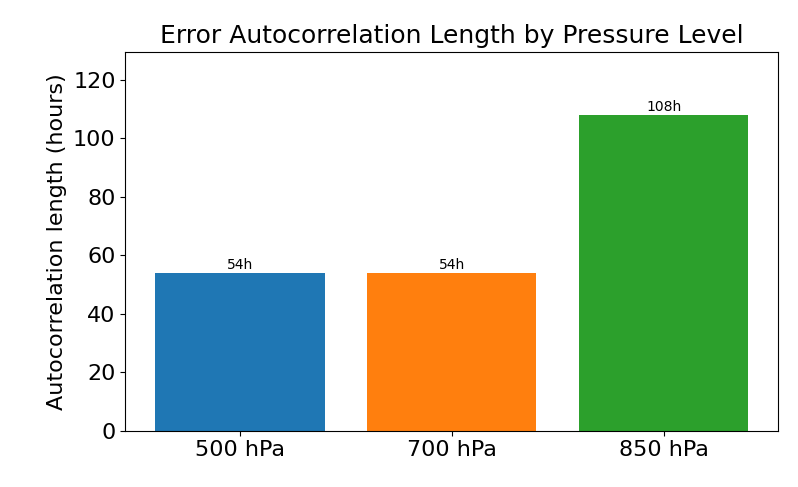
\includegraphics[width=0.7\linewidth]{Figures/autocorr_first.png}
    \caption{Autocorrelation of errors at three vertical levels indexed by pressure. Autocorrelation is higher at lower vertical levels.}
    \label{fig:autocorr}
\end{figure}

\section{Implementation details}
\label{sec:implementation_details}

The model is implemented in JAX~\cite{jax} using the Flax neural network library and the Jraph graph neural network library.
The dynamical core is provided by the Dinosaur spectral primitive equations solver.
All source code, training scripts, and analysis notebooks are available in the accompanying repository.

\subsection{Hyperparameters}

Tables~\ref{tab:hyperparams_training}--\ref{tab:hyperparams_filter} list all hyperparameters used in the experiments.

\subsubsection{Training}

\begin{table}[htbp]
\centering
\small
\begin{tabular}{lp{6.4cm}l}
\hline
\textbf{Hyperparameter} & \textbf{Description} & \textbf{Value} \\
\hline\hline
Optimiser & Gradient-based optimiser used for all runs & Adam \\
Learning rate & Base learning rate, scaled linearly by device count & $3.5 \times 10^{-4}$ \\
LR (long-range) & Reduced learning rate for prediction ranges $\geq$36\,h & $2.5$--$3.0 \times 10^{-4}$ \\
Gradient clipping & Global norm threshold for gradient clipping & 1.0 \\
NaN guard & Replaces NaN gradients with zeros via \texttt{optax.zero\_nans} & Enabled \\
Batch size & One sample per device; equals the device count & 1 per GPU \\
Training samples & Number of gradient steps per prediction-range stage & 2\,000--5\,000 \\
Validation interval & Steps between validation evaluations & 500--2\,500 \\
Epochs & Number of passes through the shuffled training set & 1 \\
Training period & ERA5 time range used for training & 2005--2018 \\
Validation period & ERA5 time range used for validation & Jan 2020 \\
Data frequency & Temporal resolution of ERA5 input/target pairs & 6-hourly \\
Random seed & Seed for parameter initialisation and data shuffling & 42 \\
Precision & Floating-point precision for all computations & float32 \\
\hline
\end{tabular}
\caption{Training hyperparameters.}
\label{tab:hyperparams_training}
\end{table}


\subsubsection{Curriculum schedule}

Training follows a curriculum strategy where the prediction horizon is progressively extended.
Each stage loads the checkpoint from the previous stage and fine-tunes toward a longer rollout.
Table~\ref{tab:curriculum} summarises the schedule used for TL47; the other resolutions follow the same structure with identical learning rates.

\begin{table}[htbp]
\centering
\small
\begin{tabular}{cccc}
\hline
\textbf{Prediction range} & \textbf{Lead time} & \textbf{Training steps} & \textbf{Learning rate} \\
\hline\hline
1 & 6\,h & 4\,000 & $3.5 \times 10^{-4}$ \\
2 & 12\,h & 2\,000 & $3.5 \times 10^{-4}$ \\
3 & 18\,h & 5\,000 & $3.5 \times 10^{-4}$ \\
4 & 24\,h & 5\,000 & $3.5 \times 10^{-4}$ \\
6 & 36\,h & 5\,000 & $3.0 \times 10^{-4}$ \\
8 & 48\,h & 5\,000 & $2.5 \times 10^{-4}$ \\
10 & 60\,h & 5\,000 & $2.5 \times 10^{-4}$ \\
\hline
\end{tabular}
\caption{Curriculum training schedule.  Each stage is initialised from the checkpoint of the previous stage.  If training diverges, the driver script falls back to the previous range with a fresh random seed.}
\label{tab:curriculum}
\end{table}

\subsubsection{Model architecture}

\begin{table}[htbp]
\centering
\small
\begin{tabular}{lp{6.4cm}l}
\hline
\textbf{Hyperparameter} & \textbf{Description} & \textbf{Value} \\
\hline\hline
GNN layers & Number of message-passing layers (excluding output layer) & 2 \\
Hidden dimensions & Width of each hidden GNN layer (resolution-dependent, see Table~\ref{tab:hidden_dims}) & 64--256 \\
Activation & Activation function in hidden layers & ReLU \\
Output activation & Activation function in the final output layer & Linear \\
Graph stencil & Neighbourhood connectivity on the nodal grid & 9-point \\
Edge aggregation & Aggregation function for incoming messages & Sum \\
Output dimension & Channels per node: $6 \times N_\text{levels} + 1$ & 79 \\
Correction factor & Multiplicative scaling of the GNN output & 0.01 \\
Vertical levels & Number of equidistant sigma levels & 13 \\
Input features & State variables provided as node features & $u, v, \zeta, D, T', \ln p_s, q$ \\
\hline
\end{tabular}
\caption{GNN correction architecture hyperparameters.}
\label{tab:hyperparams_arch}
\end{table}

\begin{table}[htbp]
\centering
\small
\begin{tabular}{lccc}
\hline
\textbf{Resolution} & \textbf{Grid (lon $\times$ lat)} & \textbf{GNN hidden dims} & \textbf{Approx.\ nodes} \\
\hline\hline
TL31  & $96 \times 49$   & $(256, 256)$ & 4\,704 \\
TL47  & $144 \times 73$  & $(176, 176)$ & 10\,512 \\
TL63  & $192 \times 97$  & $(128, 128)$ & 18\,624 \\
TL95  & $288 \times 145$ & $(80, 80)$   & 41\,760 \\
TL127 & $384 \times 193$ & $(64, 64)$   & 74\,112 \\
\hline
\end{tabular}
\caption{Per-resolution GNN hidden dimensions and grid sizes.  The hidden width is reduced at higher resolutions to keep memory usage within GPU limits.}
\label{tab:hidden_dims}
\end{table}

\subsubsection{Dynamical core and filtering}

\begin{table}[htbp]
\centering
\small
\begin{tabular}{lp{6.4cm}l}
\hline
\textbf{Hyperparameter} & \textbf{Description} & \textbf{Value} \\
\hline\hline
Time integrator & IMEX Runge--Kutta scheme for the primitive equations & SIL3 \\
$\Delta t$ & Time step for the dynamical core & 360\,s \\
Correction interval & Wall-clock interval between GNN corrections & 3\,600\,s \\
Dycore steps per correction & Number of dynamical core steps between GNN evaluations & 10 \\
DFI timescale & Digital filter initialisation window and cutoff period & 6\,h \\
Reference temperature & Background temperature profile for $T'$ decomposition & 288\,K \\
\hline
Exp.\ filter $\tau$ & Damping timescale of the exponential filter & 0.0066 \\
Exp.\ filter order & Steepness of the exponential filter rolloff & 6 \\
Exp.\ filter cutoff & Fraction of total wavenumber below which no damping occurs & 0.4 \\
Hyperdiff.\ $\tau$ & Resolution-adaptive timescale: $8.6 / 2.4^{\log_2(N_\text{lat}/64)}$\,h & Resolution-dependent \\
Hyperdiff.\ order & Order of the hyperdiffusion operator & 2 \\
GNN output filter & Exponential filter applied to the GNN correction in modal space & att.\ 8, order 6, cutoff 0.4 \\
\hline
\end{tabular}
\caption{Dynamical core and spectral filter hyperparameters.}
\label{tab:hyperparams_filter}
\end{table}

\subsection{Engineering choices}
\label{sec:engineering}

Training a hybrid model that couples a spectral dynamical core with a graph neural network on grids with up to 74\,000 nodes, 13 vertical levels, and multi-day rollouts presents substantial computational challenges.
This subsection describes the key engineering decisions that made this feasible on a small GPU cluster.

\subsubsection{Implicit JIT compilation via \texttt{pmap}}

JAX's \texttt{jax.pmap} transformation compiles the enclosed computation into an XLA program that runs identically on every device.
Because \texttt{pmap} subsumes \texttt{jit}, the entire training step---forward pass, loss computation, back-propagation, and parameter update---is compiled into a single fused XLA kernel without requiring an explicit \texttt{@jax.jit} decorator.
This fusion eliminates Python-level overhead between operations and enables the XLA compiler to perform cross-operator optimisations such as operator fusion and buffer reuse, which are critical for the memory-intensive spherical harmonic transforms in the dynamical core.

\subsubsection{Data parallelism with \texttt{pmap}}

All training, validation, and test loops use \texttt{jax.pmap} for single-program, multiple-data parallelism across GPUs.
The batch size is set equal to the number of available devices (typically 3--4 NVIDIA GPUs), so each device processes exactly one sample.
Losses and per-variable MSE metrics are synchronised across replicas with \texttt{jax.lax.pmean} before logging.
The learning rate is scaled linearly by the device count to compensate for the effective batch size, following standard practice for synchronous data parallelism.
Model parameters are replicated to all devices with \texttt{flax.jax\_utils.replicate} at the start of training and unreplicated for checkpointing.

\subsubsection{Gradient checkpointing (rematerialisation)}

The model must be differentiated through long rollout trajectories: a 24-hour forecast involves 4 outer steps, each containing 10 dynamical core time steps and one GNN evaluation.
Storing all intermediate activations for back-propagation would exceed GPU memory at higher resolutions.
To address this, we apply \texttt{jax.checkpoint} (rematerialisation) at two levels:
\begin{enumerate}
    \item \textbf{Trajectory level:} both the inner repeated-step function (\texttt{f\_repeated}) and the outer \texttt{jax.lax.scan} body are wrapped in \texttt{jax.checkpoint}, so activations are recomputed during the backward pass rather than stored.
    \item \textbf{GNN layer level:} in the three-dimensional GNN variant (\texttt{TGNNCorrection}), each \texttt{GraphNetworkLayer} and the \texttt{OutputLayer} are individually wrapped in \texttt{flax.linen.remat}, trading a modest increase in computation for a large reduction in peak memory.
\end{enumerate}
Without rematerialisation, training at TL95 and TL127 resolution would not fit in the 40\,GB memory of the available NVIDIA A100 GPUs.

\subsubsection{Scan-based trajectory rollout}

Rather than using a Python \texttt{for} loop to unroll the forecast trajectory, the model uses \texttt{jax.lax.scan} for both the inner (repeated dynamical core steps) and outer (prediction-range steps) loops.
\texttt{lax.scan} enables XLA to compile the entire rollout as a single static loop with fixed iteration count, avoiding retracing overhead and enabling the compiler to optimise memory layout across iterations.
This is combined with the rematerialisation strategy described above: \texttt{scan} provides the loop structure, while \texttt{checkpoint} controls the memory--compute trade-off within each iteration.

\subsubsection{Static graph construction}

The GNN operates on a 9-point stencil graph over the nodal grid.
Because the graph topology is fixed for a given resolution, the sender and receiver index arrays are constructed once in NumPy during model initialisation and stored as static JAX arrays.
During the forward pass, \texttt{jax.lax.stop\_gradient} is applied to the graph structure arrays to ensure they are treated as constants by the compiler and excluded from gradient computation, avoiding unnecessary memory allocation during back-propagation.

\subsubsection{Modal-space data caching}

Converting ERA5 data from the native equiangular pressure-level grid to the spectral (modal) representation on a Gaussian grid is expensive: it involves vertical interpolation from pressure to sigma coordinates, spherical harmonic transforms, and horizontal regridding.
To avoid repeating this preprocessing at every training step, the entire ERA5 training set is pre-processed offline and cached to disk in modal-space format.
The data loader then reads the cached modal states directly, reducing per-step I/O and preprocessing overhead by over an order of magnitude.

\subsubsection{Memory management}

Several additional measures keep memory usage under control:
\begin{itemize}
    \item \textbf{Lazy GPU allocation:} the XLA environment variable \texttt{XLA\_PYTHON\_CLIENT\_PREALLOCATE} is set to \texttt{false}, preventing JAX from pre-allocating the entire GPU memory at startup. This avoids out-of-memory failures when the host process also requires significant memory for data loading.
    \item \textbf{Memory fraction cap:} \texttt{XLA\_PYTHON\_CLIENT\_MEM\_FRACTION} is set to 0.85, reserving a margin for CUDA runtime and inter-process communication buffers.
    \item \textbf{Single-precision arithmetic:} all computations use float32 (\texttt{jax\_enable\_x64 = False}), halving memory consumption relative to double precision while maintaining sufficient numerical accuracy for the spectral solver.
    \item \textbf{Resolution-adaptive network width:} the GNN hidden dimension is reduced at higher resolutions (256 at TL31 down to 64 at TL127, see Table~\ref{tab:hidden_dims}), keeping the total parameter count and activation memory roughly constant across resolutions.
\end{itemize}

\subsubsection{Stability mechanisms}

Training a differentiable dynamical core through multi-step rollouts is prone to numerical instability.
The following mechanisms mitigate divergence:
\begin{itemize}
    \item \textbf{NaN-aware optimiser:} the optimiser chain includes \texttt{optax.zero\_nans()}, which replaces NaN gradients with zeros, preventing a single unstable sample from corrupting the parameters.
    \item \textbf{Best-state rollback:} if the loss becomes NaN during training, the model parameters are reverted to the last stable checkpoint (the state with the lowest observed training loss).
    \item \textbf{Curriculum fallback:} the driver script monitors the training output; if a prediction-range stage fails persistently, it automatically falls back to the previous (shorter) prediction range with a fresh random seed before retrying.
    \item \textbf{Spectral filtering of corrections:} the GNN output is filtered in modal space with an exponential filter (attenuation 8, order 6, cutoff 0.4) before being added to the dynamical core tendency, suppressing high-wavenumber noise that could trigger grid-scale instabilities.
    \item \textbf{Standard deviation normalisation:} the raw GNN output is multiplied by the per-channel standard deviation of the input state scaled by a small factor (0.01), ensuring that the initial correction magnitudes are appropriately sized relative to the dynamical tendencies.
\end{itemize}

\subsection{Training resources}

Training was performed on a SLURM-managed cluster using 3--4 NVIDIA GPUs (A100 40\,GB) per job.
A single resolution from TL31 through all curriculum stages takes approximately 12--48 hours depending on the grid size.
All training was logged to Weights \& Biases for experiment tracking and hyperparameter monitoring.
